\chapter{Teoría de Galois de Ecuaciones}
\section{Grupo de Galois de un polinomio}
\noindent
A lo largo de este capítulo, consideraremos siempre polinomios mónicos, pues solo nos interesan las raíces de los polinomios.

\begin{definicion} % El discriminante resulta ser caso particular de la resultante de dos polinomios (en particular, de un polinomio y su derivado), que es para ver si dos curvas se tocan o no, viene de la geometría clásica
    Sea $f\in F[x]$ no constante, mónico\footnote{Si no, su discriminante se define como cierto elemento de $F$ multiplicado por la cantidad enunciada, pero no será relevante pera nosotros.} y sean $\alpha_1, \ldots, \alpha_n$ sus raíces (repetidas tantas veces como indique su multiplicidad) en algún cuerpo de descomposición $K$ de $f$. Se define el \underline{discriminante} de $f$ como:
    \begin{equation*}
        \Disc(f) = \prod_{1\leq i<j \leq n} {(\alpha_i-\alpha_j)}^{2} \in K
    \end{equation*}
\end{definicion}

\noindent
Resulta que $\Disc(f)$ se puede calcular a partir de los coeficientes del polinomio.

\begin{observacion}
    Vemos que $f$ es separable $\Longleftrightarrow \Disc(f)\neq 0$. 
\end{observacion}

\begin{notacion}
    Notaremos usualmente a la raíz del discriminante $\Disc(f)$ por:
    \begin{equation*}
        \Delta(f) = \prod_{1\leq i < j \leq n}(\alpha_i-\alpha_j)
    \end{equation*}
\end{notacion}

\begin{notacion} 
    Dado un conjunto $S = \{\alpha_1, \ldots, \alpha_n\}$, denotaremos normalmente al grupo de permutaciones de dichos elementos por:
    \begin{equation*}
        \Sim(\alpha_1, \ldots, \alpha_n)
    \end{equation*}
    Observemos que $\Sim(\alpha_1,\ldots, \alpha_n)\cong S_n$.
\end{notacion}

\begin{definicion}
    Si $f\in F[x]$ es separable y $K$ es su cuerpo de descomposición, diremos que $\Aut_F(K)$ es el grupo de Galois\footnote{Observemos que por ser $f$ separable y $K$ cuerpo de descomposición suyo tenemos siempre por el Teorema~\ref{teo:piedra_angular} que la extensión $F\leq K$ es de Galois.} de $f$.
\end{definicion}

\noindent
Si $f\in F[x]$ es separable y $K$ es su cuerpo de descomposición, si consideramos $\{\alpha_1, \ldots, \alpha_n\}$ el conjunto de todas las raíces de $f$ en $K$, podemos siempre definir un homomorfismo de grupos entre el grupo de Galois de $f$ y el grupo de permutaciones de sus raíces:
\begin{align*}
    \Aut_F(K) &\longrightarrow \Sim(\alpha_1, \ldots, \alpha_n) \\
    \sigma&\longmapsto \sigma\big|_{\{\alpha_1, \ldots, \alpha_n\}}
\end{align*}
Tenemos que:
\begin{itemize}
    \item La aplicación está bien definida, pues si consideros $\sigma\in \Aut_F(K)$, tendremos siempre que $\sigma^\ast = \sigma\big|_{\{\alpha_1, \ldots, \alpha_n\}}\in \Sim(\alpha_1, \ldots, \alpha_n)$, pues si $\alpha_i$ es una raíz de $f$ (para $i \in \{1,\ldots,n\}$) tendremos entonces que $\sigma(\alpha_i)$ también es raíz de $f$:
        \begin{equation*}
            f(\sigma(\alpha_i)) = \sum_{i=0}^n f_i {(\sigma(\alpha_i))}^{i} \AstIg \sigma\left(\sum_{i=0}^{n}f_i \alpha_i^i\right) = \sigma(f(\alpha_i)) = 0
        \end{equation*}
        donde en $(\ast)$ hemos usado que $\sigma\in \Aut_F(K)$ y que $f\in F[x]$.
    \item La aplicación es un homeomorfismo, pues si $\sigma,\tau\in \Aut_F(K)$ tenemos entonces que:
        \begin{equation*}
            (\sigma\tau)\big|_{\{\alpha_1, \ldots, \alpha_n\}} = \sigma\big|_{\{\alpha_1, \ldots, \alpha_n\}}\tau\big|_{\{\alpha_1, \ldots, \alpha_n\}}
        \end{equation*}
\end{itemize}
Además dicho homomorfismo de grupos es siempre inyectivo, pues la Proposición de Extensión nos dice que cada automorfismo del grupo de Galois queda unívocamente determinado por la imagen de cada raíz de $f$, puesto que sabemos que el grupo de Galois de $f$ coincide con las extensiones de la inclusión:
\begin{equation*}
    \Aut_F(K) = Ex(\iota,\iota)
\end{equation*}
Si pensamos en la obtención de todos los elementos del grupo de Galois de $f$ mediante el siguiente procedimiento:
\begin{figure}[H]
    \centering
    \shorthandoff{""}
    \begin{tikzcd}
        F \arrow[r, hook] \arrow[rd, hook] & K                                                             & {F(\alpha_1, ..., \alpha_{i-1})} \arrow[r, hook] \arrow[rd, hook] & K                                                                              & {F(\alpha_1, ..., \alpha_{n-1})} \arrow[r, hook] \arrow[rd, hook] & K                                                 \\
                                           & F(\alpha_1) \arrow[u, "\alpha_1 \longmapsto \eta(\alpha_1)"'] &                                                                   & {F(\alpha_1, ..., \alpha_{i})} \arrow[u, "\alpha_i\longmapsto\eta(\alpha_i)"'] &                                                                   & K \arrow[u, "\alpha_n\longmapsto\eta(\alpha_n)"']
    \end{tikzcd}
    \shorthandon{""}
\end{figure}
\noindent
observamos que cada uno de ellos queda determinado por cada una de las elecciones hechas sobre cada una de las imágenes de cada raíz. De esta forma, si tenemos que dos elementos $\sigma,\tau\in \Aut_F(K)$ coinciden en $\{\alpha_1, \ldots, \alpha_n\}$, tendremos entonces que $\sigma = \tau$, lo que nos prueba la inyectividad del homomorfismo de grupos.\\

\noindent
De esta forma, como $\Sim(\alpha_1, \ldots, \alpha_n)\cong S_n$, podemos ver siempre el grupo de Galois de $f$ como subgrupo de $S_n$, aquel que permuta los índices de las raíces de $f$:
\begin{equation*}
    \alpha_i \stackrel{\sigma}{\longmapsto} \alpha_{\sigma(i)}
\end{equation*}

\begin{notacion}
    En vista de la relación existente entre $\Aut_F(K)$ (el grupo de Galois de cierto polinomio $f\in F[x]$), $\Sim(\alpha_1, \ldots, \alpha_n)$ (el grupo de permutaciones sobre sus raíces) y $S_n$, será habitual identificar $\Sim(\alpha_1, \ldots, \alpha_n)$ con $S_n$, y ver $\Aut_F(K)$ directamente como subgrupo de $S_n$. Este uso de la notación no debe llevar a errores, pues simplemente es una forma más rápida de enunciar ciertas propiedades sobre $\Aut_F(K)$.
\end{notacion}

\noindent
Una vez tenemos cierta intuición sobre el grupo de Galois $G$ de un polinomio separable, las dos siguientes Proposiciones nos ayudarán a identificar a qué subgrupo de $S_4$ es isomorfo el grupo $G$, sin necesidad de conocer los órdenes de todos los elementos del grupo, como hacíamos en el Capítulo anterior.

\begin{observacion}
    Si tomamos $\sigma\in \Aut_F(K)$, una vez visto que $\sigma$ actuando sobre las raíces del polinomio $f$ simplemente las permuta, vemos fácilmente que:
    \begin{itemize}
        \item $\sigma(\Disc(f)) = \Disc(f)$.
        \item $\sigma(\Delta(f)) = sgn(\sigma)\Delta(f)$.
    \end{itemize}
\end{observacion}

\begin{prop}\label{prop:discf}
    Sea $f\in F[x]$ separable con grupo de Galois $G = \Aut_F(K)$, entonces $\Disc(f) \in F$. Además:
    \begin{equation*}
        K^{G\cap A_n} = F(\Delta(f))
    \end{equation*}
    Por tanto, $\Delta(f) \in F \Longleftrightarrow G< A_n$.
    \begin{proof}
        Para ver que $\Disc(f)\in F$, vimos en el primer punto de la observación superior que:
        \begin{equation*}
            \sigma(\Disc(f)) = \Disc(f) \qquad \forall \sigma\in G
        \end{equation*}
        Por lo que tenemos que $\Disc(f) \in K^G$, pero como $F\leq K$ es de Galois, tenemos que $K^G = F$.\\

        \noindent
        Para ver que $K^{G\cap A_n} = F(\Delta(f))$, en vista del segundo punto de la observación superior:
        \begin{equation*}
            \sigma(\Delta(f)) = sgn(\sigma)\Delta(f) \qquad \forall \sigma\in G
        \end{equation*}
        Tenemos que $\Delta(f) \in K^{G\cap A_n}$, y como todo elemento de $G$ es $F-$lineal es claro que $F(\Delta(f)) \leq K^{G\cap A_n}$. Si estudiamos el índice de este subcuerpo de $K$, la conexión de Galois nos dice que:
        \begin{equation*}
            \left[K^{G\cap A_n} : F\right] = (G : G\cap A_n) \stackrel{(\ast)}{\leq} (S_n : A_n) = 2
        \end{equation*}
        donde en $(\ast)$ hemos usado el Segundo Teorema de Isomorfía para grupos: 
        \begin{figure}[H]
            \centering
            \shorthandoff{""}
            \begin{tikzcd}
                                              & S_n \arrow[d, no head] \arrow[rdd, "\rhd", no head]  &                         \\
                                                                            & GA_n \arrow[ld, no head] \arrow[rd, "\rhd", no head] &                         \\
                G \arrow[rd, "\rhd", no head] &                                                      & A_n \arrow[ld, no head] \\
                                              & G\cap A_n                                            &                        
            \end{tikzcd}
            \shorthandon{""}
        \end{figure}
        \noindent
        Por tanto, solo tenemos dos situaciones posibles ante $F\leq F(\Delta(f)) \leq K^{G\cap A_n}$:
        \begin{equation*}
            F(\Delta(f)) = F \qquad \text{o}\qquad F(\Delta(f)) = K^{G\cap A_n}
        \end{equation*}
        \begin{itemize}
            \item Si $F(\Delta(f)) = F$, tendremos entonces que $\Delta(f)\in F$, así como que:
                \begin{equation*}
                    sgn(\sigma)\Delta(f) = \sigma(\Delta(f)) = \Delta(f)\sigma(1) = \Delta(f)\qquad \forall \sigma\in G
                \end{equation*}
                Por lo que $G\leq A_n$, de donde:
                \begin{equation*}
                    K^{G\cap A_n} =K^G = F = F(\Delta(f))
                \end{equation*}
            \item Si $F(\Delta(f)) = K^{G\cap A_n}$, tendremos entonces que $\Delta(f)\notin F$, por lo que:
                \begin{equation*}
                    sgn(\sigma)\Delta(f) = \sigma(\Delta(f)) \neq \Delta(f)  \qquad \forall \sigma\in G
                \end{equation*}
                Por lo que $sgn(\sigma) = -1$, de donde $G\not\leq A_n$.
        \end{itemize}
    \end{proof}
\end{prop}

\noindent
En relación al enunciado de la Proposición anterior, se suele hacer referencia a la condición ``$\Delta(f)\in F$''  por ``$\Disc(f)$ es un cuadrado en $F$''. Así, tenemos que $G<A_n$ si y solo si $\Disc(f)$ es un cuadrado en $F$.

\begin{ejercicio} \label{ej:signo_disc}
    Sea $f\in \mathbb{R}[x]$ mónico con $degf = 3$, discutir el número de raíces reales de $f$ según el signo de $\Disc(f)$. \\

    \noindent
    Distinguimos casos:
    \begin{itemize}
        \item Si $\Disc(f) = 0$ tenemos entonces que $f$ tiene alguna raíz múltiple, por lo que tienen que ser todas sus raíces reales.
        \item Si $\Disc(f) < 0$, si fueran todas las raíces de $f$ reales, digamos $\alpha,\beta,\gamma\in \mathbb{R}$ tendríamos entonces que:
            \begin{equation*}
                \Disc(f) = {(\alpha-\beta)}^{2}{(\alpha-\gamma)}^{2}{(\beta-\gamma)}^{2} > 0
            \end{equation*}
            contradicción, por lo que $f$ debe tener alguna reaíz compleja $\alpha\in \mathbb{C}$, por lo que $\overline{\alpha}\in \mathbb{C}$ también es raíz y debe tener alguna raíz real.
        \item Si $\Disc(f) > 0$, si $\alpha\in \mathbb{C}\setminus\mathbb{R}$ fuera una raíz de $f$ tendríamos entonces que $\overline{\alpha}$ también sería una raíz de $f$, de donde si $\beta\in \mathbb{R}$ es la última raíz de $f$ tendríamos que:
            \begin{equation*}
                \Disc(f) = {(\alpha-\overline{\alpha})}^{2}{(\alpha-\beta)}^{2}{(\overline{\alpha}-\beta)}^{2}
            \end{equation*}
            supuesto que $\alpha = a+ib$ para $a,b\in \mathbb{R}$, tenemos entonces que:
            \begin{itemize}
                \item $\alpha-\overline{\alpha} = 2ib \quad\Longrightarrow\quad {(\alpha-\overline{\alpha})}^{2} = {(2ib)}^{2} = -4b^2 < 0$
                \item Por otra parte:
                    \begin{align*}
                        {(\alpha-\beta)}^{2}{(\overline{\alpha}-\beta)}^{2} &= {((\alpha-\beta)(\overline{\alpha}-\beta))}^{2}
                    \end{align*}
                    y tenemos que:
                    \begin{align*}
                        (\alpha-\beta)(\overline{\alpha}-\beta) &= ((a+ib)-\beta)((a-ib)-\beta) = ((a-\beta)+ib)((a-\beta)-ib) \\ &= {(a-\beta)}^{2} + b^2 > 0
                    \end{align*}
            \end{itemize}
            de donde $\Disc(f)<0$, contradicción, por lo que $f$ tiene que tener en este caso 3 raíces reales.
    \end{itemize}
\end{ejercicio}

\begin{ejemplo}
    Consideramos $f = x^n +\sum\limits_{i=0}^{n-1}a_ix^i \in F[x]$ y sean $\alpha_1, \ldots, \alpha_n$ sus raíces (repetidas según multiplicidad), tenemos que:
    \begin{equation*}
        f = \prod_{i=1}^{n}(x-\alpha_i)
    \end{equation*}
    Igualando coeficientes de igual grado, obtenemos las relaciones de Cardano-Vieta\footnote{Hay una teoría desarrollada sobre esto, siempre se obtienen funciones simétricas en las raíces del polinomio. Ver el Ejercicio~\ref{ej:cardano-vieta}}. Por ejemplo, si $n=2$ se obtiene:
    \begin{equation*}
        a_0 = \alpha_1\alpha_2 \qquad a_1 = -(\alpha_1+\alpha_2)
    \end{equation*}
    Como $\Disc(f) = {(\alpha_1-\alpha_2)}^{2}$, tenemos que $\Disc(f) = a_1^2 - 4a_0$. \newline
    Para $n>2$, la cuenta no es tan sencilla, por lo que se prefiere usar un algoritmo para resolver el sistema de ecuaciones. En definitiva, se puede expresar $\Disc(f)$ en término de los coeficientes de $f$. Para $n=3$, la damos para $f=x^3+px+q$  (cúbica reducida\footnote{Sin término cuadrático.}) es:
    \begin{equation*}
        \Disc(f) = -4p^3 - 27q^2
    \end{equation*}
\end{ejemplo}~\\

\noindent
Sea $H<S_n$, recordamos que decíamos que ``$H$ es transitivo'' si dados dos elementos cualesquiera $i,j\in \{1,\ldots,n\}$ somos capaces de encontrar $\sigma \in H$ de forma que $\sigma(i) = j$.

\begin{prop}
    Sea $f\in F[x]$ separable con grupo de Galois $G$
    \begin{equation*}
        f\text{\ es irreducible} \Longleftrightarrow G\text{\ actúa transitivamente sobre las raíces de\ } f
    \end{equation*}
    En tal caso, $degf$ divide a $|G|$.
    \begin{proof}
        Sea $K$ el cuerpo de descomposición de $f$, tenemos que $G = \Aut_F(K)$.
        \begin{description}
            \item [$\Longrightarrow )$] Si $f$ es irreducible y $\alpha,\beta\in K$ son raíces de $f$, podemos ($f = \Irr(\alpha,F)$) usar la Proposición de extensión, obteniendo $\sigma:F(\alpha)\to K$ de forma que $\sigma(\alpha) = \beta$.

                La tercera proposición de extensión nos dice que $\sigma$ puede extenderse a un automorfismo $\eta\in G$ y $\eta(\alpha) = \sigma(\alpha) = \beta$, por lo que la acción es transitiva.
            \item [$\Longleftarrow )$] Sea $g$ un factor irreducible de $f$ (ambos mónicos), tenemos que $g$ no es constante, con lo que sus raíces son también de $f$. Sea $\alpha\in K$ una raíz de $g$, tenemos que $\sigma(\alpha)$ es raíz de $g$ para todo $\sigma\in G$, y como $G$ actúa transitivamente sobre las raíces de $f$, vemos que toda raíz de $f$ también es de $g$, con lo que $f=g$, de donde $f$ es irreducible.
        \end{description}
        Finalmente, para ver que $degf$ divide a $|G|$, si $\alpha$ es raíz de $f$, tenemos entonces $[F(\alpha):F] = degf$, que divide a $[K:F]$ por el Lema de la Torre, y $|G| = [K:F]$.
    \end{proof}
\end{prop}

\begin{coro}
    Por tanto, a la hora de buscar el grupo de Galois de un polinomio irreducible, descartaremos automáticamente los subgrupos de $S_n$ no transitivos.
\end{coro}

\begin{ejemplo}
    Sea $f\in F[x]$ separable e irreducible: 
    \begin{enumerate}
        \item Si $degf = 1$, su grupo de Galois es la identidad, como único elemento de $S_1$.
        \item Si $degf = 2$, la Proposición anterior nos dice que $2 = degf$ a de dividir al cardinal del grupo, por lo que su grupo de Galois debe ser isomorfo a $C_2$ (recordemos que $S_2\cong C_2$).
        \item Si $degf = 3$, la Proposición anterior nos dice que bien $G\cong A_3$ o $G\cong S_3$, como los únicos subgrupos transitivos de $S_3$. La Proposición~\ref{prop:discf} nos dice que tenemos el primer caso si $\Delta(f)\in F$ y el segundo si $\Delta(f)\notin F$.
        \item Si $degf = 4$, la Proposición anterior nos dice que $G$ es isomorfo a un subgrupo transitivo de $S_4$. 
    \end{enumerate}
\end{ejemplo}

\subsection{Estructura de $S_n$}
\noindent
A partir del ejemplo anterior, conviene repasar ahora la estructura de $S_n$, para $n\leq 4$:
\begin{itemize}
    \item Para $S_1$ tenemos que $S_1 = \{1\}$.
    \item Para $S_2$ tenemos que $S_2 = \{1, (1\ 2)\}$.
\end{itemize}

\subsubsection{Estructura de $S_3$}
\noindent
Tenemos que $|S_3| = 3! = 6$, con:
\begin{equation*}
    S_3 = \{1, (1\ 2), (1\ 3), (2\ 3), (1\ 2\ 3), (1\ 3\ 2)\}
\end{equation*}
El Teorema de Lagrange nos dice que los subgrupos no triviales de $S_3$ tienen órdenes 2 o 3, por lo que los subgrupos no triviales de $S_3$ son aquellos generados por un único elemento, bien de orden 2 o bien de orden 3. A partir de este razonamiento y observando los elementos de $S_3$ vemos que todos los subgrupos de $S_3$ son los representados en el siguiente diagrama:
            \begin{figure}[H]
                \centering
                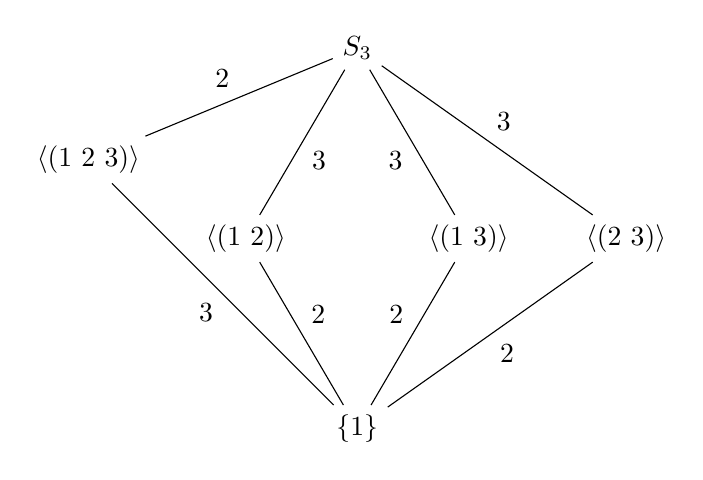
\begin{tikzpicture}[node distance=2cm]
                    \node (S3) {$S_3$};
                    \node (1) [below left of=S3, yshift=-1cm] {$\left\langle (1\ 2)\right\rangle$};
                    \node (2) [below right of=S3, yshift=-1cm] {$\left\langle (1\ 3)\right\rangle$};
                    \node (3) [left of=1, yshift=1cm] {$\left\langle (1\ 2\ 3)\right\rangle$};
                    \node (4) [right of=2] {$\left\langle (2\ 3)\right\rangle$};
                    \node (5) [below right of=1, yshift=-1cm] {$\{1\}$};
                    
                    \draw (S3) -- node[below right] {$3$} (1);
                    \draw (S3) -- node[below left] {$3$} (2);
                    \draw (S3) -- node[above left] {$2$} (3);
                    \draw (S3) -- node[above right] {$3$} (4);
                    \draw (1) -- node[above right] {$2$} (5);
                    \draw (2) -- node[above left] {$2$} (5);
                    \draw (3) -- node[below left] {$3$} (5);
                    \draw (4) -- node[below right] {$2$} (5);
                \end{tikzpicture}
                \caption{Subgrupos de $S_3$.}
            \end{figure}
\noindent
Donde tenemos que $A_3 = \langle (1\ 2\ 3) \rangle $, vemos que los subgrupos transitivos de $S_3$ son $S_3$ y $A_3$, por lo que estos son los únicos candidatos a ser grupo de Galois de un polinomio separable e irreducible de grado 3.

\subsubsection{Estructura de $S_4$}
Tenemos que $|S_4| = 4! = 24$, con:
\begin{equation*}
    S_4 = \left\{\begin{array}{l}
        1, (1\ 2), (1\ 3), (1\ 4), (2\ 3), (2\ 4), (3\ 4), (1\ 2\ 3), (1\ 3\ 2), (1\ 2\ 4), \\
        (1\ 4\ 2), (1\ 3\ 4), (1\ 4\ 3), (2\ 3\ 4), (2\ 4\ 3), (1\ 2\ 3\ 4), (1\ 3\ 2\ 4), (1\ 2\ 4\ 3), \\
    (1\ 3\ 4\ 2), (1\ 4\ 2\ 3), (1\ 4\ 3\ 2), (1\ 2)(3\ 4), (1\ 3)(2\ 4), (1\ 4)(2\ 3)
    \end{array}\right\}
\end{equation*}
El Teorema de Lagrange nos dice que los cardinales de los subgrupos de $S_4$ son divisores de $24 = 2^3\cdot 3$:
\begin{equation*}
    Div(24) = \{1, 2, 3, 4, 6, 8, 12, 24\}
\end{equation*}
Estudiamos ahora los subgrupos no triviales de $S_4$, estudiando cada divisor no trivial de 24:
\begin{description}
    \item [Subgrupos de orden 2.]~\\
        Como $2$ es primo tenemos que los subgrupos de $S_4$ de orden 2 deben ser \underline{cíclicos}, luego tenemos un subgrupo de orden 2 por cada elemento de orden 2 de $S_4$, todos ellos cíclicos, y estos son:
        \begin{equation*}
            \langle (1\ 2) \rangle , \langle (1\ 3) \rangle , \langle (1\ 4) \rangle , \langle (2\ 3) \rangle , \langle (2\ 4) \rangle , \langle (3\ 4) \rangle , \langle (1\ 2)(3\ 4) \rangle , \langle (1\ 3)(2\ 4) \rangle , \langle (1\ 4)(2\ 3) \rangle 
        \end{equation*}
        Obtenemos así $9$ subgrupos de orden 2, 6 de ellos generados por trasposiciones y 3 generados por el producto de dos trasposiciones disjuntas.

        Vemos que ninguno de estos subgrupos es transitivo.
    \item [Subgrupos de orden 3.]~\\
        Como 3 es primo, volvemos a tener tantos subgrupos de orden 3 de $S_4$ como elementos de orden 3 tiene $S_4$, por lo que estos son:
        \begin{equation*}
            \langle (1\ 2\ 3) \rangle , \langle (1\ 2\ 4) \rangle , \langle (1\ 3\ 4) \rangle , \langle (2\ 3\ 4) \rangle 
        \end{equation*}
        Obtenemos $4$ subgrupos de orden 3 (observamos que los $3-$ciclos de $S_4$ que no aparecen como generadores de un subgrupo son inversos de un $3-$ciclo que aparece como generador de un subgrupo, obteniéndose el mismo subgrupo). 

        Vemos que ninguno es transitivo.
    \item [Subgrupos de orden 4.]~\\
        Sabemos que si $H$ es un grupo de orden 4 entonces tiene que ser cíclico o isomorfo a $C_2\oplus C_2$:
        \begin{description}
            \item [Subgrupos de orden 4 cíclicos.] Estos tienen que estar generados por un elemento de orden 4, por lo que son:
                \begin{equation*}
                    \langle (1\ 2\ 3\ 4) \rangle , \langle (1\ 3\ 2\ 4) \rangle , \langle (1\ 3\ 4\ 2) \rangle 
                \end{equation*}
                Obtenemos 3 subgrupos cíclicos, todos ellos transitivos.
            \item [Subgrupos de orden 4 isomorfos a $C_2\oplus C_2$.] Sabemos que tienen que ser de la forma $\{1,a,b,ab\}$ con $O(a) = 2 = O(b)$ y $ab = ba$. Los únicos que hay de esta forma en $S_4$ son:
                \begin{itemize}
                    \item El grupo de Klein:
                        \begin{equation*}
                            V = \{1, (1\ 2)(3\ 4), (1\ 3)(2\ 4), (1\ 4)(2\ 3)\}
                        \end{equation*}
                        que es normal y transitivo.
                    \item Los generados por dos trasposiciones disjuntas, obteniendo:
                        \begin{align*}
                            \langle (1\ 2),(3\ 4) \rangle &= \{1, (1\ 2), (3\ 4), (1\ 2)(3\ 4)\} \\
                            \langle (1\ 3),(2\ 4) \rangle &= \{1, (1\ 3), (2\ 4), (1\ 3)(2\ 4)\} \\
                            \langle (1\ 4),(2\ 3) \rangle &= \{1, (1\ 4), (2\ 3), (1\ 4)(2\ 3)\}
                        \end{align*}
                        ninguno de ellos es normal o transitivo.
                \end{itemize}
        \end{description}
        Obtenemos así $7$ subgrupos de orden 4, 4 de ellos transitivos.
    \item [Subgrupos de orden 6.]~\\
        Si $H$ es un grupo de orden 6 entonces es cíclico o isomorfo a $S_3$, pero como en $S_4$ no hay elementos de orden 6 entonces los únicos subgrupos de $S_4$ que tienen orden 6 son isomorfos a $S_3$. $S_3$ es el grupo de permutaciones de un conjunto de 3 elementos $\{a,b,c\}$, por lo que subgrupos de $S_4$ de esta forma encontramos:
        \begin{gather*}
            Stab(1), \text{\ el subgrupo de permutaciones de\ } \{2, 3, 4\} \\
            Stab(2), \text{\ el subgrupo de permutaciones de\ } \{1, 3, 4\} \\
            Stab(3), \text{\ el subgrupo de permutaciones de\ } \{1, 2, 4\} \\
            Stab(4), \text{\ el subgrupo de permutaciones de\ } \{1, 2, 3\}
        \end{gather*}
        Ninguno de ellos es transitivo, puesto que todo elemento $\sigma\in Stab(i)$ verifica que $\sigma(i) = i$, para $i \in \{1,2,3,4\}$.
    \item [Subgrupos de orden 8.]~\\
        Como $|S_4| = 2^3\cdot 3$, los subgrupos de orden $8=2^3$ son los $2-$subgrpos de Sylow de $S_4$. Si notamos por $n_2$ al número de $2-$subgrpos de Sylow de $S_4$, el Segundo Teorema de Sylow nos dice que:
        \begin{equation*}
            \left.\begin{array}{c}
                n_2\equiv 1 \mod 2 \\
                n_2 \mid 3
            \end{array}\right\}  \quad\Longleftrightarrow\quad n_2 \in \{1,3\}
        \end{equation*}
        Por lo que hay uno o tres subgrupos de orden 8. Estos serán isomorfos a $C_8, C_4\oplus C_2, C_2\oplus C_2\oplus C_2, Q_8$ o $D_4$. Puede probarse que $S_4$ no tiene subgrupos isomorfos a $C_8$ (no tiene elementos de orden 8), $C_4\oplus C_2, C_2\oplus C_2\oplus C_2$ ni a $Q_8$, por lo que todos son isomorfos a $D_4$. Supuesto que $n_2 = 1$ tendríamos entonces que dicho subgrupo sería normal, pero puede probarse que esto lleva a una contradicción, por lo que $S_4$ tiene 3 subgrupos isomorfos a $D_4$. Uno de ellos es por ejemplo:
        \begin{equation*}
            \langle (1\ 3), (1\ 2\ 3\ 4) \rangle 
        \end{equation*}
        Todos ellos son transitivos.
    \item [Subgrupos de orden 12.]~\\
        Sabemos que $A_4$ es un subgrpo de $S_4$ de orden 12, que es normal y transitivo.

        Sea $H<S_4$ un subgrupo de orden 12, tenemos entonces que $(S_4:H) = 2$, por lo que $H\lhd S_4$, y tenemos que $S_4/H\cong C_2$ abeliano, por lo que $H$ debe contener el subgrupo conmutador $[S_4,S_4] = A_4$, es decir, $A_4 < H$ con $|A_4| = 12 = |H|$, por lo que $H = A_4$.

        De esta forma, $S_4$ solo tiene un único grupo de orden 12, que es $A_4$.
\end{description}
En resumen:
\begin{table}[H]
\centering
\begin{tabular}{|c|p{7.5cm}|p{3.5cm}|c|}
    \hline
    Orden & Descripción & Transitivos & Total \\
    \hline
    2 & Todos cíclicos, 6 generados por trasposiciones y 3 por dos trasposiciones disjuntas & No & 9 \\
    \hline
    3 & Todos cíclicos & No & 4 \\
    \hline
    4 & 3 cíclicos, 4 isomorfos a $C_2\oplus C_2$ y uno de estos (Klein) normal & Los cíclicos y el normal & 7 \\
    \hline
    6 & Todos isomorfos a $S_3$ & No & 4 \\
    \hline
    8 & Todos isomorfos a $D_4$ & Sí & 3 \\
    \hline
    12 & $A_4$ & Sí & 1 \\
    \hline
\end{tabular}
\caption{Subgrupos de $S_4$.}
\end{table}

\noindent
Tenemos $28$ subgrupos no triviales de $S_4$, que junto con $\{1\}$ y $S_4$ hacen un total de $30$ subgrupos. Los subgrupos transitivos de $S_4$ son:
\begin{itemize}
    \item Los tres subgrupos cíclicos de orden 4.
    \item El grupo de Klein.
    \item Los tres subgrupos isomorfos a $D_4$ de orden 8.
    \item $A_4$.
    \item $S_4$.
\end{itemize}

\noindent
Una vez repasadas las estructuras de $S_n$, terminamos esta sección con varios ejemplos y ejercicios:
\begin{ejemplo}
    Estudiando más a fondo el caso de tener $f\in F[x]$ un polinomio separable e irreducible de grado 4, sean $\alpha_1,\alpha_2,\alpha_3,\alpha_4$ las raíces de $f$ en un cuerpo de descomposición $K$ de $f$, tomamos $G=\Aut_F(K)$ y consideramos:
    \begin{align*}
        \beta_1 = \alpha_1\alpha_2 + \alpha_3 \alpha_4 \\
        \beta_2 = \alpha_1\alpha_3 + \alpha_2 \alpha_4 \\
        \beta_3 = \alpha_1\alpha_4 + \alpha_2 \alpha_3 
    \end{align*}

    y definimos:
    \begin{equation*}
        g = (x-\beta_1)(x-\beta_2)(x-\beta_3)\in K[x]
    \end{equation*}
    Veamos que en realidad $g\in F[x]$, ya que si $\sigma \in G$ podemos descomponerla como producto de trasposiciones, y cada una de ellas vemos (hágase) que permutan los elementos $\beta_i$, de donde tenemos que $g^\sigma = g\quad \forall \sigma\in G$, de donde los coeficientes de $g$ están en $K^G = F$. Este polinomio $g$ recibe el nombre \underline{resolvente cúbica de $f$}, y en general si $f = x^4+bx^3+cx^2+dx+e$, tras algunos cálculos se obtiene que:
    \begin{equation*}
        g = x^3-cx^2 + (bd-4e)x - b^2 e + 4ce - d^2
    \end{equation*}
    Y además es fácil ver que las raíces de $g$, $\beta_1,\beta_2,\beta_3$ son todas distintas, ya que por ejemplo:
    \begin{equation*}
        \beta_2 - \beta_1 = (\alpha_2 - \alpha_3)(\alpha_4-\alpha_1)
    \end{equation*}
    Y como $f$ era separable tenemos que $\beta_2-\beta_1 \neq 0$, por lo que $g$ seguirá siendo separable. Si calculamos las diferencias $\beta_3-\beta_1$ y $\beta_3-\beta_2$ veremos que tenemos que $\Disc(f) = \Disc(g)$.\\

    \noindent
    En definitiva, tenemos que $E = F(\beta_1,\beta_2,\beta_3)$ es cuerpo de descomposición de $g$ (separable), por lo que $F\leq E$ es de Galois, lo que nos dice que $N = \Aut_E(K)$ es un subgrupo normal de $G$, así como que:
    \begin{equation*}
        \Aut_F(E) \cong \frac{\Aut_F(K)}{\Aut_E(K)} = \frac{G}{N}
    \end{equation*}
    donde $\Aut_F(E)$ es el grupo de Galois de $g$.\\

    \noindent
    Para ver quién es $N$, consideramos $S:\Sim(\alpha_1,\alpha_2,\alpha_3,\alpha_4)\to\Sim(\beta_1,\beta_2,\beta_3)$ la aplicación dada por:
    \begin{equation*}
        S(\sigma)(\alpha_i\alpha_j + \alpha_k\alpha_l) = \alpha_{\sigma(i)}\alpha_{\sigma(j)} + \alpha_{\sigma(k)} \alpha_{\sigma(l)} 
    \end{equation*}
    que es un homomorfimo de grupos y es sobreyectivo (ya que dada una trasposición en el grupo de la derecha, podemos encontrar un elemento en la izquierda cuya imagen vaya a él). Para calcular su núcleo, calculamos primero su cardinal: recordamos que:
    \begin{equation*}
        |\Sim(\alpha_1,\alpha_2,\alpha_3,\alpha_4)| = 4! = 24, \qquad |\Sim(\beta_1,\beta_2,\beta_3)| = 3! = 6
    \end{equation*}
    y como $S$ es sobreyectivo, el Primer Teorema de Isomorfía de grupos nos dice que:
    \begin{equation*}
        \frac{24}{|\ker S|} = 6 \quad\Longrightarrow\quad |V| = 4
    \end{equation*}
    Si pensamos en los elementos\footnote{Aquí hacemos el abuso de pensar que $G<S_4$, ya que $S_4$ contiene un subgrupo isomorfo a $G$.} $\sigma\in G<S_4$ de forma que $S(\sigma) = id$, obtenemos que:
    \begin{equation*}
        \ker S \supseteq \{(1), (1\ 2)(3\ 4), (1\ 3)(2\ 4), (1\ 4)(2\ 3)\}
    \end{equation*}
    y como tenemos 4 elementos obtenemos que $\ker S = V$, el grupo de Klein.\\

    \noindent
    Como $F\leq E$ es de Galois, tenemos como en la demostración del Teorema~\ref{teo:normal} que $\sigma(E) = E$ para cada $\sigma\in G$, lo que nos permite considerar nuevamente (como en la demostración de dicho Teorema) el epimorfismo $r:G\to \Aut_F(E)$ dado por:
    \begin{equation*}
        r(\sigma) = \sigma\big|_E
    \end{equation*}
    obtenemos así el diagrama conmutativo:

    \begin{figure}[H]
        \centering
        \shorthandoff{""}
        \begin{tikzcd}
            V \arrow[r, hook] & {Sim(\alpha_1,\alpha_2,\alpha_3,\alpha_4)} \arrow[rr, "S"] &  & {Sim(\beta_1,\beta_2,\beta_3)} \\
            N \arrow[r, hook] & G \arrow[u] \arrow[rr, "r"']                               &  & Aut_F(E) \arrow[u]            
        \end{tikzcd}
        \shorthandon{""}
    \end{figure}
    \noindent
    Donde $V=\ker S$, $N = \ker r$ y las dos fechas verticales se identifican con el monomorfismo de grupos que ve el grupo de Galois de un polinomio dentro del grupo que permuta las raíces del polinomio.\\

    \noindent
    De aquí deducimos que (pensando nuevamente que $G<S_n$): % // TODO: Por qué?
    \begin{equation*}
        N = V\cap G
    \end{equation*}
        Ya que tomamos $\sigma\in G$ y lo vemos en $\Aut_F(E)$, las raíces $\beta$ las permutará, pero por otra parte, $\sigma$ sabe actuar sobre $\Sim(\alpha_1,\ldots,\alpha_4)$, que las permuta, y teníamos que:
        \begin{equation*}
            \beta_1 = \alpha_1\alpha_2 + \alpha_3\alpha_4
        \end{equation*}
    \begin{description}
        \item [$\subseteq )$] SI tomamos alguien de $N$ tenemos que va a la permutación trivial en $\Sim(\beta)$, pero estos están en $V$.
        \item [$\supseteq )$] Si alguien está en $G\cap V$, al aplicarle $s$ caerá en $V$, y usamos ahora que el camino es conmutativo, obteniendo que está en el núcleo de $r$.
    \end{description}
\end{ejemplo}

\begin{ejemplo} % // TODO: Terminar de entender
    Si tenemos $f=x^4+x+1\in \mathbb{Q}[x]$, no tiene raíces en $\mathbb{Q}$ (las únicas posibles son $-1$ y $1$). Como $f\in \mathbb{Z}[x]$ y $f$ es primitivo, reducimos módulo 2, obteniendo:
    \begin{equation*}
        \overline{f} = x^4+x+1 \in \mathbb{Z}_2[x]
    \end{equation*}
    $\overline{f}$ no tiene raíces y si no fuera irreducible, tendríamos entonces que sería el cuadrado del único polinomio irreducible de $\mathbb{Z}_2[x]$ que es $x^2+x+1$, pero no lo es, por lo que $f$ es irreducible sobre $\mathbb{Z}[x]$, luego sobre $\mathbb{Q}[x]$ también. Sea $G$ el grupo de Galois de $f$ sobre $\mathbb{Q}$, tenemos que $G$ es un subgrupo transitivo de $S_4$, así como que $|G|$ es un múltiplo de $degf = 4$. Los subgrupos transitivos de $S_4$ son:
    \begin{itemize}
        \item Los cíclicos de 4 elementos.
        \item El grupo de Klein.
        \item De 8 elementos tenemos los diédricos, que hay varios.
        \item $A_4$.
    \end{itemize}
    Anteriormente vimos que si $f = x^4+bx^3+cx^2+dx+e$ entonces su resolvente tenía el aspecto:
    \begin{equation*}
        g = x^3-cx^2+(bd-4e)x-b^2+4ce-d^2
    \end{equation*}
    Para nuestro polinomio $f$ su resolvente cúbica es: 
    \begin{equation*}
        g = x^3-4x -1
    \end{equation*}
    Si $\alpha_1,\alpha_2,\alpha_3,\alpha_4$ son raíces de $f$ y $\beta_1,\beta_2,\beta_3$ son las de $g$, teníamos entonces que:
    \begin{equation*}
        \beta_2-\beta_1 = (\alpha_2-\alpha_3)(\alpha_4-\alpha_1)
    \end{equation*}
    más otras dos relaciones. Usando estas, se demuestra que $\Disc(f) = \Disc(g)$. 
    Además, $g$ es una cúbica reducida, y teníamos una fórmula para calcular $\Disc(g)$, obteniendo que:
    \begin{equation*}
        \Disc(f) = \Disc(g) = -4p^3 - 27q^2 = -4{(-4)}^{3} - 27{(-1)}^{2} = 229
    \end{equation*}
    Y tenemos que $\sqrt{229}\notin \mathbb{Q}$, ya que $x^2-229\in \mathbb{Q}[x]$ es irreducible, porque $229$ es primo (se comprueba tratando de dividir entre primos hasta la parte entera de $\sqrt{229}$, que es 15). Como $\sqrt{229}\notin \mathbb{Q}$, tenemos que $G\not\subseteq A_4$, por lo que $G$ no puede ser el isomorfo a Klein ni $A_4$.\\

    \noindent
    En estas condiciones, teníamos a partir del ejemplo anterior una subextensión:
    \begin{equation*}
        \mathbb{Q}\leq E =\mathbb{Q}(\beta_1,\beta_2,\beta_3) \leq K = \mathbb{Q}(\alpha_1, \alpha_2,\alpha_3,\alpha_4)
    \end{equation*}
    Como $\mathbb{Q}\leq K$ es de Galois, tenemos que $E\leq K$ es de Galois, y la conexión nos dice que:
    \begin{equation*}
        \Aut_E(K) \lhd G
    \end{equation*}
    Veamos qué aspecto tiene $\Aut_E(K)$, para reducir las opciones sobre $G$, de hecho:
    \begin{equation*}
        \dfrac{G}{\Aut_E(K)} \cong \Aut_\mathbb{Q}(E)
    \end{equation*}
    Como $g$ no tiene raíces (ya que las únicas posibles raíces son $\pm 1$) y es de grado 3 tenemos que $g$ es irreducible, por lo que $|\Aut_\mathbb{Q}(E)|$ es múltiplo de $degg = 3$, con lo que solo puede ser 3 o 6. Como el único posible grupo $G$ que es divisible entre $3$ es la opción $G\cong S_4$. Buscamos ahora $\Aut_E(K)$, que ha de ser $V$.
\end{ejemplo}

\noindent
Respecto al tema anterior ganamos que no es necesario calcular de forma explícita cada uno de los automorfismos.

\subsection{Ejercicios}
\begin{ejercicio}\label{ej:cardano-vieta}
    (Identidades de Cardano-Vieta)\newline
    Sea $f\in F[x]$ un polinomio mónico de grado $n$ con raíces $\alpha_1,\ldots,\alpha_n$ en un cuerpo de descomposición suyo (no suponemos que $f$ sea separable, así que entre las raíces puede haber repeticiones). Definamos
    \begin{equation*}
        s_k = \sum_{1\leq i_1 < \ldots < i_k \leq n} \alpha_{i_1} \ldots \alpha_{i_k}
    \end{equation*}
    para $k \in \{1,\ldots,n\}$ se pide demostrar que:
    \begin{equation*}
        f = x^n - s_1x^{n-1} + \ldots + {(-1)}^{n}s_n
    \end{equation*}
\end{ejercicio}

\begin{ejercicio}
    Sea $f\in F[x]$ un polinomio separable e irreducible de grado primo $p$. Demostrar que el grupo de Galois de $f$ sobre el cuerpo $F$ contiene un ciclo de orden $p$.\newline
    (\textbf{Pista:} usar el Teorema de Cauchy de existencia de $p-$subgrupos)
\end{ejercicio}

\begin{ejercicio}
    Sea $f\in \mathbb{Q}[x]$ irreducible de grado primo $p$. Demostrar que, si $f$ tiene exactamente dos raíces complejas no reales, entonces el grupo de Galois de $f$ sobre $\mathbb{Q}$ es isomorfo a $S_p$.\newline
    (\textbf{Pista:} usar el Ejercicio anterior)
\end{ejercicio}

\begin{ejercicio}
    Demostrar que el grupo de Galois de $f= x^5-4x-1\in \mathbb{Q}[x]$ es isomorfo a $S_3$.
\end{ejercicio}

\begin{ejercicio}
    Sea $f\in \mathbb{R}[x]$ un polinomio de grado 3. Discutir el número de raíces reales de $f$ en función del signo de su discriminante.\\

    \noindent
    Se hizo ya en el Ejercicio~\ref{ej:signo_disc}.
\end{ejercicio}

\section{Extensiones ciclotómicas}
\noindent
Para $n\geq 1$, a lo largo de este capítulo nos interesará el polinomio $x^n-1\in F[x]$, para $F\leq K$ cualquier extensión.
\begin{prop}
    Si $n\geq 1$ y consideramos como $S$ el conjunto de todas las raíces de $x^n-1\in F[x]$ en $K$ para $F\leq K$ cualquier extensión, tenemos que $S$ es un subgrupo cíclico de $K^\times$ cuyo orden es un divisor de $n$.
    \begin{proof}
        Para ver que $S<K^\times$, sean $\alpha,\beta\in S$, tenemos que:
        \begin{equation*}
            \alpha^n - 1 = 0 = \beta^n -1 \quad \Longrightarrow \quad  \alpha^n = 1 = \beta^n
        \end{equation*}
        Y observamos ahora que:
        \begin{equation*}
            {(\alpha\beta^{-1})}^{n} -1  = (\alpha^n \beta^{-n})-1 = (1\cdot 1) - 1 = 0
        \end{equation*}
        Por lo que $\alpha\beta^{-1}\in S$, de donde $S$ es un subgrupo de $K^\times$. Sabemos que $S$ es un subgrupo cíclico de $K^\times$ por el Ejercicio~\ref{ej:subgrupo_finito}, ya que $S$ tiene como mucho $n$ elementos. Además, su orden ha de dividir a $n$, pues todos los elementos tienen orden un divisor de $n$, ya que $\alpha^n = 1 \quad \forall \alpha\in S$.
    \end{proof}
\end{prop} 

\noindent
Además, si $x^n-1\in F[x]$ es separable y $K$ contiene un cuerpo de descomposición suyo, entonces $S$ contiene todas las $n$ raíces de $x^n-1$ y todas estas son distintas, por lo que tenemos que $|S| = n$. Esto motiva a trabajar siempre en esta sección en un cuerpo $F$ en el que $x^n-1\in F[x]$ sea separable.

\begin{definicion}
    Si $x^n-1\in F[x]$ es separable y $K$ es su cuerpo de descomposición:
    \begin{itemize}
        \item Llamamos \underline{raíces $n-$ésimas de la unidad sobre $F$} a las raíces de $x^n-1$, que se encuentran en $K$.

            Las raíces $n-$ésimas de la unidad forman un subgrupo cíclico de $K^\times$ de orden $n$, a cuyos generadores llamaremos \underline{raíces $n-$ésimas primitivas de la unidad}.

            Así, un elemento $\alpha\in K$ es raíz $n-$ésima de la unidad sobre $F$ si y solo si tiene orden multiplicativo un divisor de $n$. En el caso de que el orden sea exactamente $n$ tenemos que $\alpha$ es una raíz $n-$ésima primitiva de la unidad sobre $F$.
        \item Decimos que $K$ es la $n-$ésima extensión ciclotómica de $F$.

            De esta forma, si $\zeta$ es una raíz $n-$ésima primitiva de la unidad sobre $F$, tenemos que $K = F(\zeta)$.
    \end{itemize}
    Muchas veces omitiremos el cuerpo $F$ (es decir, no especificaremos ``sobre $F$'' o ``de $F$''), entendiendo que queda claro por el contexto.

    Además, siempre que hagamos referencia a ``raíces $n-$ésimas de la unidad'', supondremos de forma implícita que $x^n-1\in F[x]$ es separable.
\end{definicion}

\begin{ejemplo}
    Si tomamos $F=\mathbb{Q}$ (observamos que $x^n-1\in \mathbb{Q}[x]$ es separable), tenemos que las raíces $n-$ésimas de la unidad sobre $\mathbb{Q}$ son las raíces complejas $n-$ésimas de la unidad que ya conocíamos, se trata del grupo cíclico:
    \begin{equation*}
        \left\{e^{i\frac{2\pi k}{n}} : k \in \{0,1,\ldots,n-1\}\right\} \cong \mathbb{Z}_n
    \end{equation*}
    Vemos que $e^{i\frac{2\pi}{n}}$ es una raíz $n-$ésima primitiva de la unidad sobre $\mathbb{Q}$, por lo que $\mathbb{Q}\left(e^{i\frac{2\pi}{n}}\right)$ es la $n-$ésima extensión ciclotómica de $\mathbb{Q}$.
\end{ejemplo}

\begin{ejemplo}
    Sea $\zeta$ cualquier raíz $n-$ésima primitiva de la unidad sobre $F$, tenemos que el conjunto de raíces $n-$ésimas de la unidad viene dado por:
    \begin{equation*}
        \left\{\zeta^k : k\in \mathbb{Z}_n\right\}
    \end{equation*}
    Y en Álgebra I vimos que $|\cc{U}(\mathbb{Z}_n)| = \varphi(n)$, donde $\varphi$ es la función de Euler, por lo que el conjunto de raíces $n-$ésimas primitivas de la unidad sobre $F$ es:
    \begin{equation*}
        \left\{\zeta^k : k\in \cc{U}(\mathbb{Z}_n)\right\}
    \end{equation*}
\end{ejemplo}

\begin{observacion}
    Si $\zeta$ es una raíz $n-$ésima primitiva de la unidad sobre $F$, hemos visto que la $n-$ésima extensión ciclotómica de $F$ es $F(\zeta)$, y vemos ahora que:
    \begin{equation*}
        [F(\zeta):F] \leq n-1
    \end{equation*}
    ya que $x^n-1\in F[x]$ es un polinomio del que $\zeta$ es raíz, pero es divisible por $x-1$ (ya que $1$ es raíz de $x^n-1$), por lo que $deg\Irr(\zeta,F)\leq n-1$.
\end{observacion}

\begin{ejercicio}
    Si $\zeta$ es una raíz $n-$ésima primitiva de la unidad sobre $F$ y $\sigma$ es un elemento del grupo de Galois de la $n-$ésima extensión ciclotómica de $F$, entonces $\sigma(\zeta)$ es una raíz $n-$ésima primitiva de la unidad.\\

    \noindent
    Tenemos que $\sigma \in G$, donde $G = \Aut_F(F(\zeta))$. Si tomamos $f = x^n-1\in F[x]$, vemos que $G$ es el grupo de Galois de $f$, y en el capítulo anterior vimos que entonces $\sigma$ permuta las raíces de $f$, por lo que $\sigma(\zeta)$ es una raíz $n-$ésima de la unidad.\\

    \noindent
    Por reducción al absurdo, supongamos que $\sigma(\zeta)$ no es una raíz $n-$ésima primitiva de la unidad, por lo que tiene que tener un orden multiplicativo menor estricto que $n$, luego existe $1\leq d < n$ de forma que:
    \begin{equation*}
        {(\sigma(\zeta))}^{d} = 1
    \end{equation*}
    Pero como $\sigma$ es un automorfismo tenemos entonces que:
    \begin{equation*}
        \sigma\left(\zeta^d\right) = {(\sigma(\zeta))}^{d} = 1 = \sigma(1) \quad\Longrightarrow\quad \zeta^d = 1
    \end{equation*}
    donde hemos usado la inyectividad de $\sigma$, llegando a contradicción, pues el orden de $\zeta$ es $n$ al ser una raíz $n-$ésima primitiva. La contradicción viene de suponer que $\sigma(\zeta)$ no es una raíz $n-$ésima primitiva de la unidad.
\end{ejercicio}

\begin{prop}\label{prop:grupo_galois_ciclotomico}
    Si $G$ es el grupo de Galois de la $n-$ésima extensión ciclotómica de $F$, entonces $G$ es isomorfo a un subgrupo de $\cc{U}(\mathbb{Z}_n)$.\newline
    Además, $G$ es isomorfo a $\cc{U}(\mathbb{Z}_n)$ si y solo si $G$ actúa transitivamente sobre las raíces $n-$ésimas primitivas de la unidad sobre $F$.
    \begin{proof}
        Sea $\zeta$ una raíz $n-$primitiva de la unidad sobre $F$, tenemos que:
        \begin{equation*}
            G = \Aut_F(F(\zeta))
        \end{equation*}
        Hemos visto que las raíces $n-$ésimas primitivas de la unidad sobre $F$ son:
        \begin{equation*}
            \{\zeta^k : k\in \cc{U}(\mathbb{Z}_n)\}            
        \end{equation*}
        Observamos ahora que si tomamos $\sigma\in G$ tenemos por el Ejercicio anterior que $\sigma(\zeta)$ debe ser una raíz $n-$ésima primitiva de la unidad sobre $F$, por lo que ha de existir $k\in \cc{U}(\mathbb{Z}_n)$ de forma que $\sigma(\zeta)=\zeta^k$. Esto nos permite definir una aplicación $G\to \cc{U}(\mathbb{Z}_n)$ dada por:
        \begin{equation*}
            \sigma \longmapsto k
        \end{equation*}

        donde $k$ queda unívocamente determinado por la condición:
        \begin{equation*}
            \sigma(\zeta) = \zeta^k
        \end{equation*}
        Si $\sigma,\tau\in G$ de forma que $\tau(\zeta) = \zeta^l$, $\sigma(\zeta)=\zeta^k$ con $l,k\in \cc{U}(\mathbb{Z}_n)$, tenemos que:
        \begin{equation*}
            \sigma\tau(\zeta) = \sigma(\zeta^l) = \sigma(\zeta)^l = {(\zeta^k)}^{l} = \zeta^{kl} 
        \end{equation*}
        Por lo que la aplicación considerada es un homomorfismo de grupos, que además es inyectivo ya que cada $\sigma$ está determinado por su valor sobre $\zeta$, gracias a la Proposición de extensión. Tenemos pues que $G$ es isomorfo a la imagen de $G$ por dicho monomorfismo, subgrupo de $\cc{U}(\mathbb{Z}_n)$.\\

        \noindent
        Observamos que el homomorfismo enunciado será sobreyectivo si y solo si para cada $k\in \cc{U}(\mathbb{Z}_n)$ existe $\sigma \in G$ de forma que $\sigma(\zeta) = \zeta^k$, condición equivalente a que $G$ actúe transitivamente sobre las raíces $n-$ésimas primitivas de la unidad sobre $F$.
    \end{proof}
\end{prop}

\begin{definicion}
    Sea $F$ un cuerpo, definimos el \underline{$n-$ésimo polinomio ciclotómico} como:
    \begin{equation*}
        \phi_n = \prod_{k\in \cc{U}(\mathbb{Z}_n)} \left(x-\zeta^k\right)
    \end{equation*}
    donde $\zeta$ es una raíz $n-$ésima primitiva de la unidad sobre $F$. Observamos que $deg\phi_n = |\cc{U}(\mathbb{Z}_n)| = \varphi(n)$.
\end{definicion}

\begin{prop}\label{prop:formula_ciclotomico}
    Se tiene que:
    \begin{equation*}
        x^n-1 = \prod_{d \in Div(n)}\phi_d
    \end{equation*}
    \begin{proof}
        Consideramos como $R_n$ el conjunto de todas las raíces $n-$ésimas de la unidad, con lo que: 
        \begin{equation*}
            x^n - 1 = \prod_{\alpha \in R_n}(x-\alpha)
        \end{equation*}
        Si para cada $m\geq 1$ consideramos también $P_m$, el conjunto de las raíces $m-$ésimas primitivas de la unidad, obtenemos una partición de $R_n$:
        \begin{equation*}
            R_n = \biguplus_{d\in Div(n)}P_d
        \end{equation*}
        \begin{description}
            \item [$\supseteq)$] Si $\alpha \in P_d$ para $d\in Div(n)$ tenemos entonces que el orden multiplicativo de $\alpha$ es exactamente $d$, divisor de $n$, luego $\alpha \in R_n$.
            \item [$\subseteq)$] Si $\alpha \in R_n$ tenemos que el orden multiplicativo de $\alpha$ es cierto natural $k$, con $k\mid n$ y es claro que $\alpha \in P_k$.
        \end{description}
        Vemos así que cada $\alpha\in R_n$ está en un cierto $P_d$ con $d\in Div(n)$, por lo que el monomio $(x-\alpha)$ ha de estar en un único (puesto que la unión es disjunta) $\phi_d$, con lo que:
        \begin{equation*}
            x^n - 1 = \prod_{\alpha \in R_n}(x-\alpha) = \prod_{d\in Div(n)}\phi_d
        \end{equation*}
    \end{proof}
\end{prop}

\begin{observacion}
    Si $F\leq K$ con $f,g\in F[x]$, $h\in K[x]$ con $f = hg$, entonces $h \in F[x]$.
    \begin{proof}
        Si dividimos $f$ entre $g$ en $F[x]$ obtenemos $q,r\in F[x]$ con $degr < degg$ y $f = qg+r$. Sin embargo, como también tenemos que $q,r\in K[x]$ y el cociente y resto en el anillo de polinomios de un cuerpo son únicos, tiene que ser $r=0$ y $q=h$, por lo que en particular $h\in F[x]$.
    \end{proof}
\end{observacion}

\begin{prop}
    Cada $\phi_n$ tiene coeficientes en el subcuerpo primo de $F$. Además, si $\car(F) = 0$, tenemos que $\phi_n\in \mathbb{Z}[x]$.
    \begin{proof}
        Si $\Pi$ es el subcuerpo primo de $F$, por inducción sobre $n$:
        \begin{itemize}
            \item Si $n=1$, entonces $\phi_1 = x-1$ y se tiene la Proposición.
            \item Si $n>1$, tenemos por la Proposición anterior que:
                \begin{equation*}
                    x^n-1 = \phi_n \cdot \prod_{\substack{d \in Div(n)\\d<n}}\phi_d
                \end{equation*}
                Por hipótesis de inducción, tenemos que cada $\phi_d$ tiene coeficientes en $\Pi$, por lo que el producto de la derecha también los tendrá. Si vemos ahora $\phi_n$ como cociente de $x^n-1$ entre dicho producto, como estos dos tienen coeficientes en $\Pi$, $\phi_n$ también ha de tener sus coeficientes en $\Pi$, por la observación anterior.
        \end{itemize}
        Si $\car(F) = 0$, procedemos nuevamente por inducción sobre $n$, tratando de probar además que cada $\phi_n$ es primitivo:
        \begin{itemize}
            \item Si $n=1$, $\phi_1 = x-1$, se tiene.
            \item Si $n>1$, sabemos por lo ya probado que $\phi_n \in \mathbb{Q}[x]$. Si expresamos sus coeficientes como fracciones irreducibles y tomamos $a\in \mathbb{Z}$ el mínimo común múltiplo de sus denominadores, obtenemos que $a\phi_n \in \mathbb{Z}[x]$ con todos sus coeficientes coprimos entre sí, luego $a\phi_n$ es primitivo. Si usamos nuevamente la Proposición anterior, tenemos que:
                \begin{equation*}
                    a(x^n-1) = a\phi_n \prod_{\substack{d\in Div(n)\\d<n}}\phi_d
                \end{equation*}
                Por hipótesis de inducción tenemos que cada $\phi_d$ es primitivo, por lo que por el Lema de Gauss\footnote{Visto en Álgebra I, el producto de polinomios primitivo es primitivo.} tenemos que $a(x^n-1)$ es primitivo, por ser igual al producto de la derecha. Luego $a=1$ (en realidad sería $a\in \{\pm 1\}$, pero en este caso sirve tanto $1$ como $-1$), lo que significa que $\phi_n$ tenía en realidad sus coeficientes en $\mathbb{Z}$. Vemos (para seguir la inducción) que $\phi_n$ es primitivo, ya que $\phi_n = a\phi_n$.
        \end{itemize}
    \end{proof}
\end{prop}

\begin{ejemplo}
    En característica cero: 
    \begin{itemize}
        \item $\phi_1 = x-1$, ya que $1$ es la única raíz de $x-1$, por lo que es una 1-raíz primitiva de 1.
        \item $\phi_2 = x+1$, ya que $\{\pm 1\}$ es el conjunto de raíces de $x^2-1$, y $-1$ es la única con orden multiplicativo dos.
        \item $\phi_3 = x^2+x+1$, ya que $\{1,w,w^2\}$ es el conjunto de las raíces cúbicas de la unidad, y tanto $w$ como $w^2$ son generadores, por lo que $\phi_3$ es el cociente tras dividir $x^3-1$ entre $x-1$.
        \item $\phi_4 = x^2+1$, ya que $\{\pm 1, \pm i\}$ es el conjunto de las raíces de $x^4-1$ y $i,-i$ son las dos raíces cuárticas primitivas de la unidad.
    \end{itemize}
    Para $\phi_6$ usamos la fórmula vista en la Proposición~\ref{prop:formula_ciclotomico}:
    \begin{equation*}
        x^6-1 =\prod_{d\in Div(6)}\phi_d =  \phi_1\phi_2\phi_3\phi_6 \quad\Longrightarrow\quad\phi_6 = \frac{x^6-1}{\phi_1\phi_2\phi_3} = x^2-x+1
    \end{equation*}
    Nos ahorramos así tener que calcular las raíces sextas primitivas de la unidad complejas y realizar la multiplicación de los monomios, pero a cambio tenemos que recordar la fórmula y realizar varias divisones de polinomios.
\end{ejemplo}

\begin{ejercicio}
    Calcular en característica cero $\phi_8$.\\

    \noindent
    Si aplicamos la fórmula de la Proposición~\ref{prop:formula_ciclotomico}, tenemos que:
    \begin{equation*}
        \phi_8 = \frac{x^8-1}{\prod_{\substack{d\in Div(8)\\ d < 8}} \phi_d} = \frac{x^8-1}{\phi_1\phi_2\phi_4}
    \end{equation*}
    y sabemos que $\phi_1 = x-1$, $\phi_2=x+1$ y $\phi_4 = x^2+1$, por lo que:
    \begin{equation*}
        \phi_1\phi_2\phi_4 = (x-1)(x+1)(x^2+1) = (x^2-1)(x^2+1) = x^4-1
    \end{equation*}
    vemos que:
    \begin{equation*}
        x^8-1 = (x^4-1)(x^4+1)
    \end{equation*}
    por lo que $\phi_8 = x^4+1$.
\end{ejercicio}

\begin{teo}
    Cada polinomio ciclotómico $\phi_n\in \mathbb{Z}[x]$ es irreducible.
    \begin{proof}
        Sea $f\in \mathbb{Z}[x]$ un factor irreducible de $\phi_n$, tomamos $\zeta$ cualquier raíz compleja de $f$ en la $n-$ésima extensión ciclotómica. Veamos que si $p$ es un primo que no divide a $n$ entonces $\zeta^p$ es también raíz de $f$. Por reducción al absurdo, si $\zeta^p$ no es raíz de $f$ entonces debe ser raíz de cierto polinomio $g\in \mathbb{Z}[x]$ con:
        \begin{equation*}
            \phi_n = fg\qquad f,g\in \mathbb{Z}[x]
        \end{equation*}
        Por lo que $\zeta$ es raíz de $h=g(x^p)\in \mathbb{Z}[x]$. De esta forma, $f$ y $h$ tienen una raíz común compleja, y la identidad de Bezout nos dice entonces que $f$ y $h$ no son coprimos. Como $f$ es irreducible, ha de ser $f\mid h$, y como $f$ además es primitivo, tenemos que $f\mid h$ en $\mathbb{Z}[x]$. Reducimos módulo $p$, obteniendo: 
        \begin{equation*}
            \overline{\phi_n} = \overline{f}\overline{g}
        \end{equation*}

        y que:
        \begin{equation*}
            \overline{h} = \overline{g(x^p)} \AstIg {\overline{g(x)}}^{p} = \overline{g}^p
        \end{equation*}
        donde en $(\ast)$ usamos que como ${(a+b)}^{p} = a^p + b^p$ en un cuerpo de característica $p$, entonces si $g = \sum a_i x^i$ tenemos entonces que (usando que $a^p = a$ para $a \in \bb{F}_p$):
        \begin{equation*}
            \overline{g(x)}^p = {\left(\sum a_i x^i\right)}^{p} = \sum {(a_ix^i)}^{p} = \sum a_i^p {(x^i)}^{p} = \sum a_i {(x^i)}^{p} = \overline{g(x^p)}
        \end{equation*}
        Como $\overline{f}$ divide a $\overline{h} = \overline{g}^p$, tenemos entonces que $\overline{f}$ y $\overline{g}$ han de tener un factor común en $\bb{F}_p[x]$, cierto polinomio $d\in \bb{F}_p[x]$, luego $\overline{x^n-1} = x^n-1\in \bb{F}_p[x]$ tiene a $d^2$ como factor en el anillo de polinomios de su cuerpo de descomposición, de donde $x^n-1\in \bb{F}_p[x]$ tiene alguna raíz múltiple. Pero esto no es posible, ya que como $p$ no divide a $n$ tenemos que el polinomio derivado de $x^n-1$ es $nx^{n-1} \neq 0$, y este no comparte raíces con $x^n-1$, luego es separable en $\bb{F}_p[x]$. Hemos llegado a una contradicción, por lo que por cada primo $p$ que no divide a $n$ tenemos que $\zeta^p$ es raíz de $f$.\\

        \noindent
        Si tomamos ahora $\zeta$ una raíz de $f$, como $f$ dividía a $\phi_n$ vemos que $\zeta$ es una raíz $n-$ésima primitiva de la unidad. Sea $\eta$ cualquier raíz $n-$ésima primitiva de la unidad, existe $k \in \mathbb{Z}_n$ con $\mcd(n,k)=1$ (ya que $\eta$ es raíz primitiva de la unidad) de forma que $\eta = \zeta^k$, y si descomponemos $k$ como producto de primos:
        \begin{equation*}
            k = p_1 p_2 \ldots p_n
        \end{equation*}
        vemos que ninguno de estos primos puede dividir a $n$, ya que $\mcd(n,k)=1$. Como $\zeta$ es raíz de $f$ y $p_1$ es un primo que no divide a $n$, tenemos que $\zeta^{p_1}$ es también una raíz de $f$, y aplicando de nuevo que $p_2$ es un primo que no divide a $n$, vemos que ${(\zeta^{p_1})}^{p_2} = \zeta^{p_1p_2}$ es una raíz de $f$. En una cantidad finita de pasos obtenemos que $\zeta^{p_1p_2 \ldots p_n} = \zeta^k = \eta$ es una raíz de $f$, por lo que acabamos de ver que cada raíz $n-$ésima primitiva de la unidad es también raíz de $f$, en caso de que $f$ tenga alguna raíz. De aquí vemos que ha de ser $f = \phi_n$, por lo que $\phi_n$ es irreducible, para cada $n\geq 1$.
    \end{proof}
\end{teo}

\begin{coro}
    El grupo de Galois de la $n-$ésima extensión ciclotómica sobre $\mathbb{Q}$ es isomorfo a $\cc{U}(\mathbb{Z}_n)$, por lo que:
    \begin{equation*}
        [\mathbb{Q}(\zeta):\mathbb{Q}] = \varphi(n)
    \end{equation*}
    donde $\zeta$ es una raíz $n-$ésima primitiva de la unidad sobre $\mathbb{Q}$.
    \begin{proof}
        Sea $\zeta$ una raíz $n-$ésima primitiva de la unidad, tenemos que el grupo de Galois de la $n-$ésima extensión ciclotómica sobre $\mathbb{Q}$ es:
        \begin{equation*}
            \Aut_\mathbb{Q}(\mathbb{Q}(\zeta)) = \Aut(\mathbb{Q}(\zeta))
        \end{equation*}
        a partir del Teorema anterior vemos que $\phi_n = \Irr(\zeta,\mathbb{Q})$, por lo que:
        \begin{equation*}
            |\Aut(\mathbb{Q}(\zeta))| = [\mathbb{Q}(\zeta):\mathbb{Q}] = \deg \phi_n = \varphi(n)
        \end{equation*}
        Y usando la Proposición~\ref{prop:grupo_galois_ciclotomico} vemos que $\Aut(\mathbb{Q}(\zeta))$ debe ser isomorfo a $\cc{U}(\mathbb{Z}_n)$.
    \end{proof}
\end{coro}

\noindent
Vemos además por la Proposición~\ref{prop:grupo_galois_ciclotomico} que el grupo de Galois de la $n-$ésima extensión ciclotómica sobre $\mathbb{Q}$ actúa transitivamente sobre las raíes $n-$ésimas primitivas de la unidad sobre $\mathbb{Q}$, es decir, sobre las raíces de $\phi_n$.

\begin{ejemplo} % // TODO: HACER
    Para $n=16$, tenemos: 
    \begin{equation*}
        \deg \phi_n = \varphi(16) = 8
    \end{equation*}
    Si $\zeta\in \mathbb{C}$ es una raíz decimosexta primitiva de la unidad tenemos que la decimosexta extensión ciclotómica de $\mathbb{Q}$ es $K=\mathbb{Q}(\zeta)$, con:
    \begin{equation*}
        \Aut(K) \cong \cc{U}(\mathbb{Z}_{16})
    \end{equation*}
    Por el último Corolario vemos que:
    \begin{equation*}
        \Aut(K) = \{\tau_j: j \in \cc{U}(\mathbb{Z}_{16})\}
    \end{equation*}
    donde cada automorfismo viene determinado por $\tau_j(\zeta) = \zeta^j$. Se ve que $\Aut(K) = \langle \tau_3,\tau_7 \rangle $, y se obtiene que el conjunto de subgrupos de $\Aut(K)$ es:
    \begin{figure}[H]
        \centering
        \shorthandoff{""}
        \begin{tikzcd}
                                                         &                                                                        & {\langle \tau_3, \tau_7\rangle} \arrow[d, no head] \arrow[ld, no head] \arrow[rd, no head] &                                           \\
                                                                                                      & {\langle \tau_7, \tau_9\rangle} \arrow[ld, no head] \arrow[d, no head] & \langle \tau_3\rangle \arrow[d, no head]                                                   & \langle \tau_5\rangle \arrow[ld, no head] \\
            \langle \tau_{15}\rangle \arrow[rd, no head] & \langle \tau_7\rangle \arrow[d, no head]                               & \langle \tau_9\rangle \arrow[ld, no head] \arrow[lu, no head]                              &                                           \\
                                                         & \langle \tau_1\rangle                                                  &                                                                                            &                                          
        \end{tikzcd}
        \shorthandon{""}
    \end{figure}

    \noindent
    Y por la conexión de Galois obtenemos que los subcuerpos de $\mathbb{Q}(\zeta)$ son:
    \begin{figure}[H]
        \centering
        \shorthandoff{""}
        \begin{tikzcd}
                                                               &                                                                         & \mathbb{Q} \arrow[d, no head] \arrow[ld, no head] \arrow[rd, no head] &                                         \\
                                                                                                                  & \mathbb{Q}(\zeta^2 + \zeta^{14}) \arrow[ld, no head] \arrow[d, no head] & \mathbb{Q}(\zeta^2 + \zeta^6) \arrow[d, no head]                      & \mathbb{Q}(\zeta^4) \arrow[ld, no head] \\
            \mathbb{Q}(\zeta + \zeta^{15}) \arrow[rd, no head] & \mathbb{Q}(\zeta^3 + \zeta^5) \arrow[d, no head]                        & \mathbb{Q}(\zeta^2) \arrow[ld, no head] \arrow[lu, no head]           &                                         \\
                                                               & \mathbb{Q}(\zeta)                                                       &                                                                       &                                        
        \end{tikzcd}
        \shorthandon{""}
    \end{figure}
\end{ejemplo}

\section{Construcciones con regla y compás II} % // TODO: Arreglar la sección
\noindent
Con objetivo de resolver el problema de cuándo es construible un polígono regular mediante regla y compás, complementaremos el Teorema~\ref{teo:torres_raices}. Para ello, dado un conjnto $S$ de números complejos en el que $\{0,1\}\subseteq S$, consideraremos $F = \mathbb{Q}(S\cup \overline{S})$.

\begin{teo} % // TODO: Arreglar
    Sea $z\in \mathbb{C}$, tenemos que $z$ es constructible a partir de $S$ si, y solo si, existe una extensión de Galois $F\leq K$ tal que $z\in K$ y $[K:F] = 2^k$, para $k\geq 1$.
    \begin{proof}
        Por doble implicación:
        \begin{description}
            \item [$\Longrightarrow )$] Sé que existe una torre de subcuerpos de $\mathbb{C}$:
                \begin{equation*}
                    F=F_0\leq F_1\leq \ldots \leq F_s
                \end{equation*}
                tales que $F_{i+1} = F(\alpha_{\alpha_i+1})$, con $\alpha_{i+1}^2 \in F_i$, para todo $i \in \{0,\ldots,s-1\}$; con $z\in F_s$. Por inducción sobre $s$:
                \begin{itemize}
                    \item Para $s=0$, tenemos que $F_s = F_0$, por lo que tomamos $K = F_0$, que trivialmente es de Galois.
                    \item Supongamos como hipótesis de inducción que existe una extensión de Galois $F\leq E$ con grado una potencia de $2$ y tal que $F_{s-1}\leq E$. Llamamos $a_s = \alpha_s^2\in F_{s-1}$, y enumeramos los elementos:
                        \begin{equation*}
                            \Aut_F(E) = \{\sigma_0, \ldots, \sigma_t\}
                        \end{equation*}
                        Y definimos el polinomio:
                        \begin{equation*}
                            f = \prod_{j=0}^{t} (x^2-\sigma_j(a_s))
                        \end{equation*}
                        Que resulta ser un polinomio con coeficientes en $E$, pero queda fijo por cualquier automorfismo de la extensión de Galois, por lo que en realidad tenemos que $f\in F[x]$.

                        \noindent
                        Como $F\leq E$ es de Galois, tenemos que $E$ es cuerpo de descomposición de cierto $g\in F[x]$. Tomamos como $K$ el cuerpo de descomposición de $fg$, por lo que $F\leq K$ es de Galois. Definimos $\alpha_{s+j}$ como la raíz de $x^2-\sigma_j(a_s)$, para cada $j \in \{0, \ldots, t\}$, por lo que $\alpha_{s+j}\in K$.

                        \noindent
                        Tenemos que:
                        \begin{equation*}
                            K = E(\alpha_s, \alpha_{s+1}, \ldots,\alpha_{s+t})
                        \end{equation*}
                        Puesto que las raíces de $g$ ya están en $E$. Como el grado de $\alpha_{s+j}$ es 1 o 2 (al ser raíz de $x^2-\alpha_j(a_s)$), tenemos que $F\leq K$ tiene grado una potencia de 2. Ahora, como $F_s\leq K$, tenemos que $z\in F_s\leq K$, para completar la inducción.
                \end{itemize}
            \item [$\Longleftarrow )$] Tomamos $z\in K$ con $F\leq K$ de Galois y $[K:F]$ una potencia de $2$. Tenemos por tanto que $\Aut_F(K)$ es un $2-$grupo, luego es resoluble\footnote{Por ser un $p-$grupo.}. Podemos por tanto tomar una serie de composición suya, obteniendo:
                \begin{equation*}
                    \Aut_F(K) = G_0 \geq G_1 \geq \ldots \geq G_n = \{id\}
                \end{equation*}
                con factores de composición $2$. La conexión de Galois nos transforma esta cadena en una cadena de extensiones de subcuerpos cuadráticas:
                \begin{equation}\label{eq:torre}
                    F=K_0 \leq K_1 \leq \ldots \leq K_n = K
                \end{equation}
                con $[K_{i+1}:K_i] = 2$, para cada $i \in \{0, \ldots, n-1\}$, por lo que:
                \begin{equation*}
                    K_{i+1} = K_i(\beta_i)\qquad \text{con}\qquad \beta_i = \frac{-b_i\pm \sqrt{b_i^2 - 4c_i}}{2}
                \end{equation*}
                en el caso de que $\Irr(\beta_i,K_i) = x^2+b_ix+c_i$. De esta forma:
                \begin{equation*}
                    K_{i+1} = K_i\left(\sqrt{b_i^2 - 4c_i}\right)
                \end{equation*}
                Por tanto, tenemos que~(\ref{eq:torre}) es una torre por raíces cuadradas, con lo que $z$ es constructible a partir de $S$.
        \end{description}
    \end{proof}
\end{teo}

% // TODO: Hay un ejemplo que no tengo copiado

Sabemos que el heptágono no es constructible, puesto que $\Irr(\sqrt[7]{algo},\mathbb{Q})$ es de grado 6, al ser $\varphi(7) = 6$, que no es una potencia de 2.

\begin{coro}
    Un polígono regular de $n$ lados es constructible (con regla y compás) si y solo si $\varphi(n)$ es una potencia de 2.
    \begin{proof}
        Decir que un polígono regular de $n$ lados es constructible es equivalente a decir que una raíz primitiva $n-$ésima de la unidad sobre $\mathbb{Q}$ es constructible. Por tanto, hemos de ver que $\zeta$ es constructible (como raíz $n-$ésima primitiva de la unidad) si y solo si $\varphi(n)$ es una potencia de 2.
        \begin{description}
            \item [$\Longrightarrow )$] Si $\zeta$ es constructible, existe una extensión de Galois $\mathbb{Q}\leq K$ de grado 2 que contiene a $\zeta$, luego ha de contener a la $n-$ésima extensión ciclotómica de $\mathbb{Q}$: $\mathbb{Q}\leq \mathbb{Q}(\zeta)\leq K$, de donde por el Lema de la Torre ha de ser $\varphi(n)$ una potencia de 2.
            \item [$\Longleftarrow )$] Si $\varphi(n)$ es una potencia de 2, como $[\mathbb{Q}(\zeta):\mathbb{Q}] = \varphi(n)$, tenemos entonces que $\mathbb{Q}\leq \mathbb{Q}(\zeta)$ es una extensión de Galois de grado una potencia de 2, por lo que $z$ es constructible.
        \end{description}
    \end{proof}
\end{coro}

De esta forma:
\begin{table}
\centering
\begin{tabular}{c|c}
    $n$ & Es constructible \\
    \hline
    3 & Sí \\
    4 & Sí \\
    5 & Sí \\
    6 & Sí \\
    7 & No \\
    8 & Sí \\
    9 & No \\
    10 & Sí \\
    11 & No \\
    12 & No \\
    13 & No \\
    14 & No \\
    15 & Sí \\
    16 & Sí \\
    17 & Sí \\
\end{tabular}
\caption{Qué polígonos regulares son constructibles.}
\end{table}

\noindent
Si $n$ es primo, tenemos que $\varphi(n) = n-1$, que es una potencia de 2 si y solo si el primo es de la forma $2^{algo}+1$. Haciendo la cuenta, tiene que ser:
\begin{equation*}
    n = 2^{2^m} + 1
\end{equation*}
\begin{itemize}
    \item $m=0$, 3
    \item $m=1$, 5
    \item $m=2$, 17
    \item $m=3$, algo
    \item $m=4$, 65 mil y pico
\end{itemize}
Sin embargo, todavía no se ha encontrado un primo más de esta forma, los llamados primos de Fermat

